\appendix

\chapter{Anexe}

\section{Figuri}

\begin{figure}[h]
	\centering
	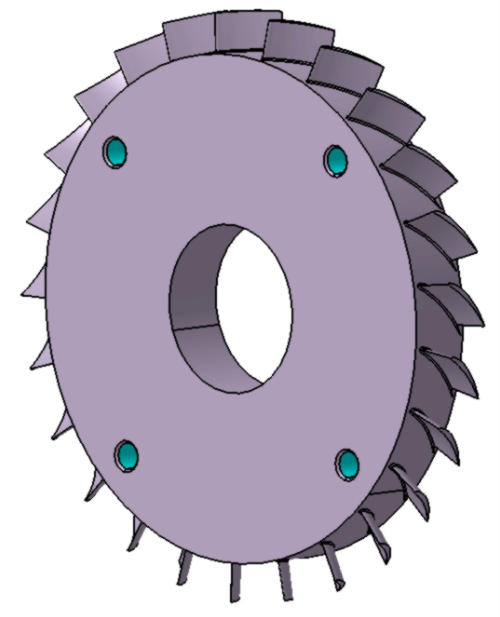
\includegraphics[scale=0.4]{figures/stator-CAD.PNG}
	\caption{Stator}
	\label{Stator}
\end{figure}

\begin{figure}[h]
	\centering
	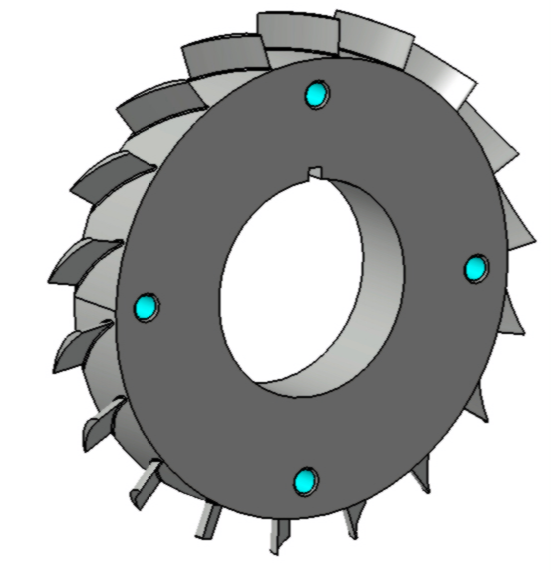
\includegraphics[scale=0.4]{figures/rotor-CAD.PNG}
	\caption{Rotor}
	\label{Rotor}
\end{figure}

\clearpage


\begin{figure}[h]
	\centering
	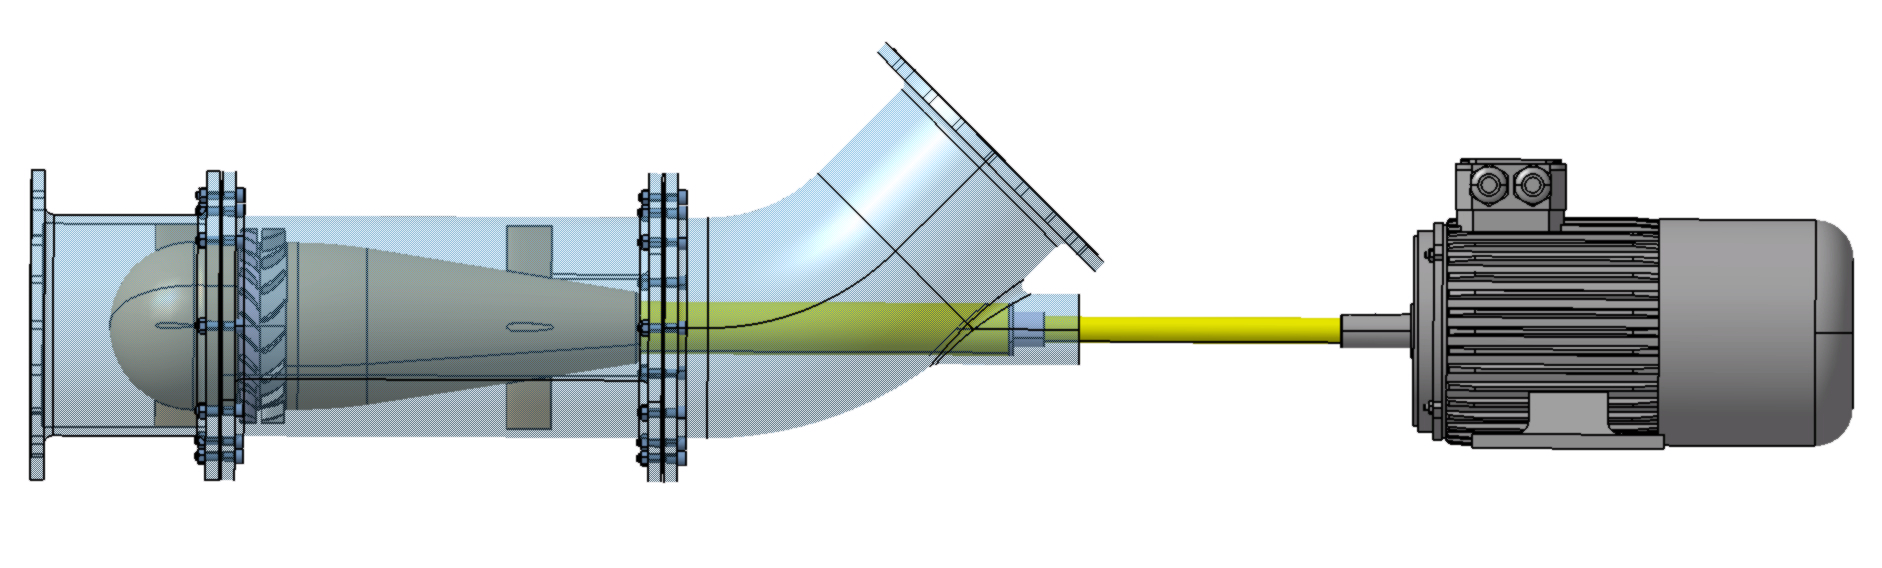
\includegraphics[scale=0.4, angle = -90]{figures/assy.jpg}
	\caption{Ansamblu turbină AXENT}
	\label{Ansamblu turbină AXENT}
\end{figure}

\clearpage


\section{Programe Fortran de calcul}

\subsection{Rezolvarea ecuației polinomiale cubice}

\lstinputlisting[language=Fortran]{code/free-swirl-stag.for}

\clearpage


\subsection{Setarea rețelei și a formei inițiale a paletei}

\lstinputlisting[language=Fortran]{code/bladesetup.for}

\clearpage


\subsection{Corecția iterativă a formei și pantei paletei subțiri}

\lstinputlisting[language=Fortran]{code/bladeupdate.for}

\clearpage


\subsection{Calculul modulului vitezei pe fețele paletei}

\lstinputlisting[language=Fortran]{code/bladevelocity.for}

\clearpage


\begin{comment}
\subsection{Subrutina de calcula a valorii minime a unei funcții cu variabile multiple}

\lstinputlisting[language=Fortran]{code/bobyqa.for}

\clearpage
\end{comment}


\subsection{Design pentru paleta subțire cu o viteză maximă minimă}

\lstinputlisting[language=Fortran]{code/thinbladecascade.for}

\clearpage


\subsection{Adăugare funcție de grosime}

\lstinputlisting[language=Fortran]{code/thickblade.for}

\clearpage


\section{Prezentare lucrare științifică}

Pe paginile următoare se găsește lucrarea științifică pregătită pentru CIEM 2019. Prezentarea acesteia are loc în 17-18 Octombrie la Timișoara în categoria Hydro Power Engineering.

Conferința Internațională pentru Energie și Mediu (CIEM) este organizată de Academia Oamenilor de Știință din România, Universitatea POLITEHNICA din București, Universitatea Politehnica din Timișoara în parteneriat cu Consiliul Mondial al Energiei - Comitetul Național Român. A 9-a Conferință Internațională privind Energia și Mediul (CIEM) este co-sponsorizată tehnic de către Societatea IEEE Power & Energy.

Obiectivele CIEM sunt de a răspunde provocărilor din domeniile în curs de dezvoltare rapidă ale Ingineriei Energetice și Ingineria Mediului și de a inspira studiile de cercetare și aplicațiile practice prin promovarea interacțiunii dintre oamenii de știință din universități, instituții de cercetare și industrie.

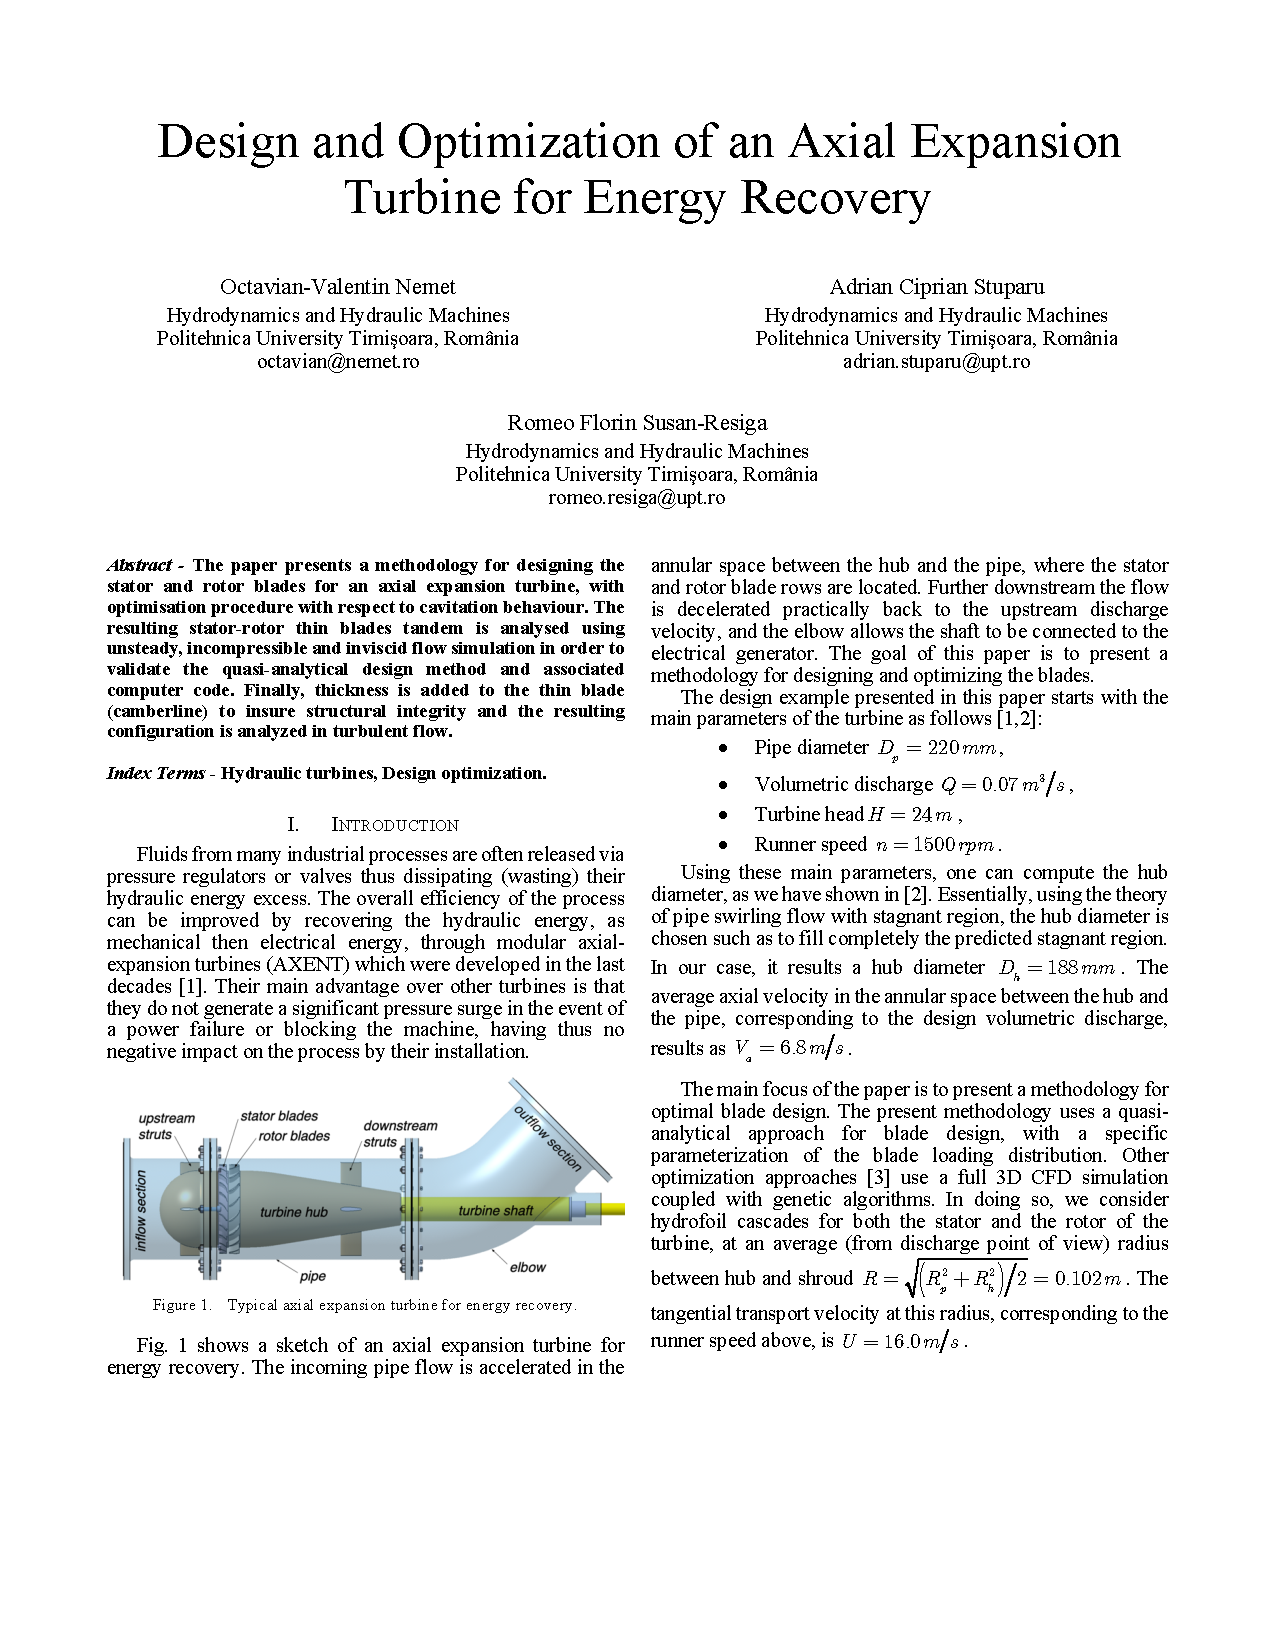
\includepdf[pages={1-}]{pages/AXENT_CIEM2019_Full_Paper_rev08.pdf}

\clearpage